
%%%%%%%%%%%%%%%%%%%%%%%%%%%%%%%%%%%%%%%%%%%%%%%%%%%%%%%%%%
%%
%% This is the "PREAMBLE". Here we define the type of document and load in any packages we might want. You can also set parameters %% % and create your own short-hand here.
%%
%%%%%%%%%%%%%%%%%%%%%%%%%%%%%%%%%%%%%%%%%%%%%%%%%%%%%%%%%%

 \documentclass[9pt]{article}
 
 \def\solutions{1}


 \usepackage{amsmath}
 \usepackage{amssymb}
 \usepackage{graphicx}    % needed for including graphics e.g. EPS, PS \usepackage{tikz}
 \usepackage{tikz}\usetikzlibrary{calc,arrows.meta}
 \usepackage{tikzsymbols}
 \usepackage{relsize}
 \usetikzlibrary{patterns,decorations.pathreplacing,shapes,arrows}
 \usepackage{algorithm2e}
 \topmargin -2.5cm        % read Lamport p.163
 \oddsidemargin -0.04cm   % read Lamport p.163
 \evensidemargin -0.04cm  % same as oddsidemargin but for left-hand pages
 \textwidth 16.59cm
 \textheight 25.94cm
% \pagestyle{empty}        % Uncomment if don't want page numbers
 \pagenumbering{gobble}
 \parskip 7.2pt           % sets spacing between paragraphs
 %\renewcommand{\baselinestretch}{1.5} 	% Uncomment for 1.5 spacing between lines
 \parindent 0pt		  % sets leading space for paragraphs

% No date in header
\date{}

\usepackage{hyperref}
\hypersetup{
    colorlinks=true,
    linkcolor=blue,
    filecolor=magenta,      
    urlcolor=cyan,
}
\usepackage{amsthm}
\usepackage{fancyhdr}
\pagestyle{fancy}
\setlength{\headsep}{36pt}

\usepackage{hyperref}

\newcommand{\lp}{\left(}
\newcommand{\rp}{\right)}
\newcommand{\lb}{\left[}
\newcommand{\rb}{\right]}
\newcommand{\ls}{\left\{}
\newcommand{\rs}{\right\}}
\newcommand{\lbar}{\left|}
\newcommand{\rbar}{\right|}
\newcommand{\ld}{\left.}
\newcommand{\rd}{\right.}

\newcommand{\myexists}{\exists \hspace{.3mm}}

\newcommand{\hs}{\hspace{.75mm}}
\newcommand{\bs}{\hspace{-.75mm}}
\newcommand{\nin}{\noindent}

\newcommand{\fx}{f\bs\left( x \right)}
\newcommand{\gx}{g\bs\left( x \right)}
\newcommand{\qx}{q\bs\left( x \right)}

\newcommand{\nn}{\nonumber}

\newcommand{\vfive}{\vspace{5mm}}
\newcommand{\vthree}{\vspace{3mm}}

\newcommand{\fof}[1]{f\lp #1\rp}
\newcommand{\gof}[1]{g\lp #1\rp}
\newcommand{\qof}[1]{q\lp #1\rp}

\newcommand{\myp}[1]{\left( #1 \right)}
\newcommand{\myb}[1]{\left[ #1 \right]}
\newcommand{\mys}[1]{\left\{ #1 \right\}}
\newcommand{\myab}[1]{\left| #1 \right|}

\newcommand{\myj}{_j}
\newcommand{\myjp}{_{j+1}}
\newcommand{\myjm}{_{j-1}}

\newcommand{\f}[1]{f\hspace{-1mm}\left( #1 \right)}
\newcommand{\fp}[1]{f'\hspace{-1mm}\left( #1 \right)}
\newcommand{\g}[1]{g\hspace{-1mm}\left( #1 \right)}
\newcommand{\gp}[1]{g'\hspace{-1mm}\left( #1 \right)}
\newcommand{\q}[1]{q\hspace{-1mm}\left( #1 \right)}
\newcommand{\qp}[1]{q'\hspace{-1mm}\left( #1 \right)}
\newcommand{\Px}[1]{P\hspace{-1mm}\left( x_{#1} \right)}
\newcommand{\Qx}[1]{Q\hspace{-1mm}\left( x_{#1} \right)}

\newcommand{\tten}[1]{\times 10^{#1}}

\newcommand{\aij}[1]{a_{#1}}
\newcommand{\bij}[1]{b_{#1}}
\newcommand{\rij}[1]{r_{#1}}

\newcommand{\R}[1]{\mathbb{R}^{#1}}

\newcommand{\ith}{i^{\textrm{th}}}
\newcommand{\jth}{i^{\textrm{th}}}
\newcommand{\kth}{i^{\textrm{th}}}

\newcommand{\inv}[1]{{#1}^{-1}}

\newcommand{\bx}{\mathbf{x}}
\newcommand{\bv}{\mathbf{v}}
\newcommand{\bw}{\mathbf{w}}
\newcommand{\by}{\mathbf{y}}
\newcommand{\bb}{\mathbf{b}}
\newcommand{\be}{\mathbf{e}}
\newcommand{\br}{\mathbf{r}}
\newcommand{\xhat}{\hat{\mathbf{x}}}

\newcommand{\beq}{\begin{eqnarray}}
\newcommand{\eeq}{\end{eqnarray}}

\newcommand{\ben}{\begin{enumerate}}
\newcommand{\een}{\end{enumerate}}

\newcommand{\bsq}{\mathsmaller{\blacksquare}}

\newcommand{\iter}[1]{^{\myp{#1}}}

% matrix macro
\newcommand{\mymat}[1]{
\left[
\begin{array}{rrrrrrrrrrrrrrrrrrrrrrrrrrrrrrrrrrrrrrr}
#1
\end{array}
\right]
}

\newcommand{\makenonemptybox}[2]{%
%\par\nobreak\vspace{\ht\strutbox}\noindent
\item[]
\fbox{% added -2\fboxrule to specified width to avoid overfull hboxes
% and removed the -2\fboxsep from height specification (image not updated)
% because in MWE 2cm is should be height of contents excluding sep and frame
\parbox[c][#1][t]{\dimexpr\linewidth-2\fboxsep-2\fboxrule}{
  \hrule width \hsize height 0pt
  #2
 }%
}%
\par\vspace{\ht\strutbox}
}
\makeatother

\newcommand{\smallaug}[1]{
\left[
\begin{array}{rr|r}
#1
\end{array}
\right]
}

\tikzset{
	vertex/.style={circle,draw,minimum size=16, inner sep=0pt,font=\normalsize},
	every node/.style={draw=none,rectangle,font=\scriptsize,outer sep=0pt,inner sep=2pt},
	directed/.style={arrows={-Stealth[length=7pt]},font=\small},
	caption/.style={text width=6cm,align=center,rectangle,draw}
	}
\newcounter{dummy}
\newcommand\myitem[1][]{\item[#1]\refstepcounter{dummy}\def\@currentlabel{#1}}

%%%%%%%%%%%%%%%%%%%%%%%%%%%%%%%%%%%%%%%%%%%%%%%%%%%%%%%%%%
%%
%% End of PREAMBLE
%%
%%%%%%%%%%%%%%%%%%%%%%%%%%%%%%%%%%%%%%%%%%%%%%%%%%%%%%%%%%



% ======================================================================================
% Actual document starts here. 
% PLEASE FILL IN YOUR NAME AND STUDENT ID.
% ======================================================================================
\begin{document}

\lhead{{\bf CSCI 3104, Algorithms \\ Problem Set 8 (50 points)} }
\rhead{Name: \fbox{YOUR NAME HERE} \\ ID: \fbox{YOUR STUDENT ID HERE} \\ {\bf Due March 19, 2021 \\ Spring 2021, CU-Boulder}}
\renewcommand{\headrulewidth}{0.5pt}

\phantom{Test}

\begin{small}
\textit{Advice 1}:\ For every problem in this class, you must justify your answer:\ show how you arrived at it and why it is correct. If there are assumptions you need to make along the way, state those clearly.
\vspace{-3mm} 

\textit{Advice 2}:\ Verbal reasoning is typically insufficient for full credit. Instead, write a logical argument, in the style of a mathematical proof.\\
\vspace{-3mm} 

\textbf{Instructions for submitting your solution}:
\vspace{-5mm} 

\begin{itemize}
	\item The solutions \textbf{should be typed} and we cannot accept hand-written solutions. \href{http://ece.uprm.edu/~caceros/latex/introduction.pdf}{Here's a short intro to Latex.}
	\item You should submit your work through \href{https://www.gradescope.com/courses/218966}{\textbf{Gradescope}} only.
	\item The easiest way to access Gradescope is through our Canvas page. There is a Gradescope button in the left menu.
	\item Gradescope will only accept \textbf{.pdf} files.
	\item \href{https://www.youtube.com/watch?v=u-pK4GzpId0&feature=emb_logo}{It is vital that you match each problem part with your work.} Skip to 1:40 to just see the matching info.
\end{itemize}
\vspace{-4mm} 
\end{small}

\hrulefill
\pagebreak



\ben

%%%%%%%%%%%%%%%%%%%%%%%%%%%%%%%%%%%%%%%%%%%%%%%%%%%%%%%%
% PROBLEM ONE %% PROBLEM ONE %% PROBLEM ONE %% PROBLEM ONE %% PROBLEM ONE %
%==============================================================================
% Problem 1: generic algorithm/GENERIC-MST
%==============================================================================
% PROBLEM ONE %% PROBLEM ONE %% PROBLEM ONE %% PROBLEM ONE %% PROBLEM ONE %
%%%%%%%%%%%%%%%%%%%%%%%%%%%%%%%%%%%%%%%%%%%%%%%%%%%%%%%%

\vspace{5mm}

\item 
We know it is important to find a safe edge in the generic minimum spanning tree algorithm. Consider the undirected, weighted graph $G$ shown below. The bold edges represent (the edges of) an intermediate spanning forest $F$, obtained by running the generic minimum spanning tree algorithm. The intermediate spanning forest $F$ has three components: $\{a,b,h\}$, $\{g,f\}$ and $\{c,d,e\}$.
For each non-bold edge in the graph, determine whether the edge is \textbf{safe}, \textbf{useless} or \textbf{undecided}.  
\begin{center}
	\begin{tikzpicture}[
		wide/.style={line width=4pt},
		vertex/.style={circle,draw,minimum size=16},
		scale=4]
                \node[vertex] (h) at (0,1) {$h$};
		\node[vertex] (a) at (0,0) {$a$};
		\node[vertex] (b) at (1,0) {$b$};
		\node[vertex] (c) at (2,1) {$c$};
		\node[vertex] (d) at (3,0.5) {$d$};
		\node[vertex] (g) at (1,-1) {$g$};
		\node[vertex] (f) at (2,-1) {$f$};
		\node[vertex] (e) at (3,-1) {$e$};
		\draw[wide] (a) to [edge label'=2] (b); 
		\draw (a) to [edge label'=8] (c); 
		\draw (b) to [edge label'=9] (c); 
		\draw[wide] (c) to [edge label'=1] (d); 
		\draw[wide] (d) to [edge label'=3] (e); 
		\draw (c) to [edge label'=4] (e); 
		\draw (c) to [edge label'=12] (f);
		\draw[wide] (g) to [edge label'=6] (f);
		\draw (g) to [edge label'=10] (a);   
                \draw[wide] (h) to [edge label'=1] (a);
                \draw(h) to [edge label'=7] (c);
                \draw(h) to [edge label'=70] (b);
\end{tikzpicture}
\end{center}

\if\solutions1
\vspace{2mm}

\textbf{Solution:} \\
%==============================================================================
% STUDENTS: TYPE YOUR SOLUTIONS HERE. (Between \textbf{Solution:} and \fi )
%==============================================================================


\fi
\newpage


%%%%%%%%%%%%%%%%%%%%%%%%%%%%%%%%%%%%%%%%%%%%%%%%%%%%%%%%
% PROBLEM TWO %% PROBLEM TWO %% PROBLEM TWO %% PROBLEM TWO %% PROBLEM TWO %
%==============================================================================
% Problem 2: max flow/min cut
%==============================================================================
% PROBLEM TWO %% PROBLEM TWO %% PROBLEM TWO %% PROBLEM TWO %% PROBLEM TWO %
%%%%%%%%%%%%%%%%%%%%%%%%%%%%%%%%%%%%%%%%%%%%%%%%%%%%%%%%


\vspace{5mm}

\item \textbf{5 points extra credit to those who use Latex/Tikz to write up each step in their solution for Problems 2 and 3. You may hand draw your solution for this problem, however to receive the bonus points, you must have your solution nicely and neatly Latexed (we recommend Tikz).}

For both parts of Problem 2, use the following flow network. 

\begin{center}
	\begin{tikzpicture}[scale=1.6]
		\node[vertex] (s) at (1,1) {$s$};
		\node[vertex] (u) at (2,2) {$u$};
		\node[vertex] (v) at (2,0) {$v$};
		\node[vertex] (w) at (3.5,2) {$w$};
		\node[vertex] (x) at (3.5,0) {$x$};
		\node[vertex] (t) at (4.5,1) {$t$};
	
		\draw[directed] (s) to [edge label =6] (u);
		\draw[directed] (s) to [edge label'=3] (v);
		\draw[directed] (u) to [edge label =2] (v);
		\draw[directed] (u) to [edge label =2] (w);
		%\draw[directed] (v) to [edge label =2,pos=0.4] (t);
		\draw[directed] (v) to [edge label'=2] (x);
		\draw[directed] (v) to [edge label =3] (w);
		\draw[directed] (w) to [edge label =3] (t);
		\draw[directed] (w) to [edge label =8] (x);
		\draw[directed] (x) to [edge label'=2] (t);
	\end{tikzpicture}
\end{center}

\begin{enumerate}
	\myitem[(2a)]\label{2a}
	Using the Ford--Fulkerson algorithm, compute the maximum flow that can be pushed from $s$ to $t$, using $s \to u \to w \to t$ as your first augmenting path.

	In order to be eligible for full credit you must include the following:
	\begin{itemize}
	\item The residual network for each iteration, including the residual capacity of each edge. 
	\item The flow augmenting path for each iteration, including the amount of flow that is pushed through this path from $s \to t$.
	\item The updated flow network \textbf{after each iteration}, with flows for each directed edge clearly labeled.
	\item The maximum flow being pushed from $s \to t$ after the termination of the Ford-Fulkerson algorithm.
	\end{itemize}
\end{enumerate}

\begin{enumerate}
	\myitem[(2b)]\label{2b} The Ford--Fulkerson algorithm terminates when there is no longer an augmenting path on the residual network. At this point, you can find a minimum cut of the form $(S,T)$ where $s\in S$ and $t\in T$. Indicate this cut and its value.
\end{enumerate}


\if\solutions1
\vspace{2mm}

\textbf{Solution:} \\

% Special Note! If you use Tikz to demonstrate your answer on Problems 2 AND 3 you'll receive +5 bonus points on this assignment! You are permitted to hand-draw your solution to this problem and the next one and upload an image of your written work. However, only nicely LaTexed solutions will receive the bonus points. 
%==============================================================================
% STUDENTS: TYPE YOUR SOLUTIONS HERE. (Between \textbf{Solution:} and \fi )
%==============================================================================

\fi

\newpage

%%%%%%%%%%%%%%%%%%%%%%%%%%%%%%%%%%%%%%%%%%%%%%%%%%%%%%%%
% PROBLEM THREE %% PROBLEM THREE %% PROBLEM THREE %% PROBLEM THREE %% PROBLEM THREE %
%==============================================================================
% Problem 3: bipartite matching
%==============================================================================
% PROBLEM THREE %% PROBLEM THREE %% PROBLEM THREE %% PROBLEM THREE %% PROBLEM THREE %
%%%%%%%%%%%%%%%%%%%%%%%%%%%%%%%%%%%%%%%%%%%%%%%%%%%%%%%%


\vspace{5mm}

\item  \textbf{5 points extra credit to those who use Latex/Tikz to write up each step in their solution for Problems 2 and 3. You may hand draw your solution for this problem, however to receive the bonus points, you must have your solution nicely and neatly Latexed (we recommend Tikz).}

A video game store is selling video games to different customers. Each of the customers only has the money to buy at most one video game. Due to the low storage of the video games, each of the different video games only has one copy available for sale. The video game store decides to run an algorithm to make sure the maximum number of customers can buy the game. \\
Example - Following is one such preference of each customer. If the games all get sold according to customers' first preference, only 3 games will be sold. But a better sale strategy is Alice - {\it AFL}, Bob - {\it Dark}, Carol - {\it Cars}, Dave - {\it Exit}, Elize - {\it Fuel}, Frank - {\it Backbreaker} and this gets 6 game sold. \\

Help them come up with an algorithm to find a sale strategy that gets the maximum games sold using Ford-Fulkerson.
\begin{figure}[h!]
\begin{center}
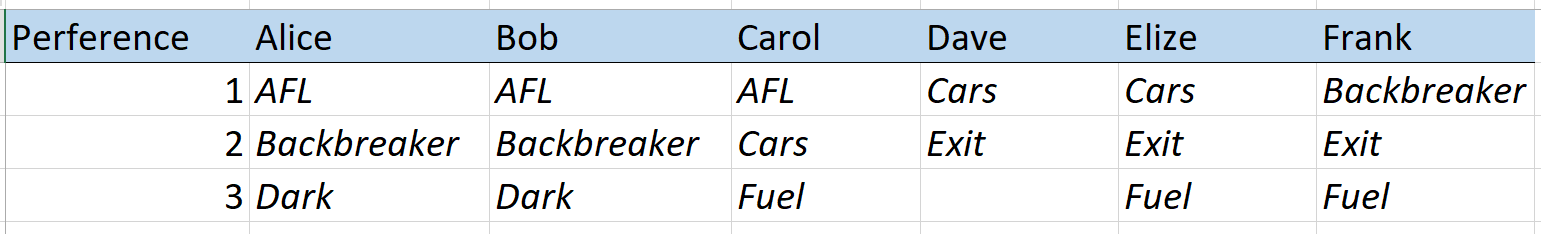
\includegraphics[scale=0.5]{Game.png}
\end{center}
\end{figure}

\begin{enumerate}
    \item Draw a network $G$ to represent this problem as a flow maximization problem for the example given above. Clearly indicate the source, the edge directions, the sink/target, and the capacities, and label the vertices.

    
    \item Assume that you have access to Fork-Fulkerson sub-routine called \textbf{Ford-Fulkerson(G)} that takes a network and gives out max-flow in terms of f(e) for all the edges. How will you use this sub-routine to find the maximum games sold. Clearly explain your solution.

\end{enumerate}

\if\solutions1
\vspace{3mm}
{\bf Solution}: \\

% Special Note! If you use Tikz to demonstrate your answer on Problems 2 AND 3 you'll receive +5 bonus points on this assignment! You are permitted to hand-draw your solution to this problem and the previous one and upload an image of your written work. However, only nicely LaTexed solutions will receive the bonus points. 
%==============================================================================
% STUDENTS: TYPE YOUR SOLUTIONS HERE. (Between \textbf{Solution:} and \fi )
%==============================================================================


\fi


%========================================================================================================================

\een 


\end{document}
